\documentclass{book}
\usepackage[paperwidth=148mm,paperheight=35mm,text={148mm,160mm},left=0mm,top=10pt]{geometry}
\usepackage{ctexcap}
\usepackage[labelfont=bf,labelsep=quad]{caption}
  \DeclareCaptionFont{kai}{\kaishu}
  \captionsetup{textfont=kai}
\usepackage{graphicx,floatrow}
\renewcommand{\rmdefault}{ptm}
\begin{document}
\setcounter{chapter}{2}

\begin{figure}[!h]
\begin{floatrow}
\captionsetup{labelsep=newline,justification=raggedleft}
\floatsetup{capbesideposition=left}
\fcapside[\FBwidth]{\caption{CPW �ṹ������ͼ}}{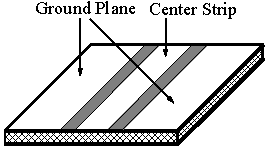
\includegraphics{fig4.pdf}}
\captionsetup{justification=raggedright}
\floatsetup{capbesideposition=right}
\fcapside[\FBwidth]{\caption{SRR-CPW ������ʾ��ͼ}}{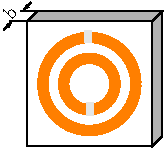
\includegraphics{fig5.pdf}}
\end{floatrow}
\end{figure}
\end{document}
